\documentclass[12pt,english]{scrbook}

\usepackage[utf8]{inputenc} % Required for inputting international characters
\usepackage[T1]{fontenc}  % These options actually change the Font!!!!
\usepackage{lmodern} 	 %..which we can suppress by this package if we like to!

\usepackage{fontspec}

\setsansfont[
BoldFont=cmunbsr.otf,
ItalicFont=cmunbmo.otf,
BoldItalicFont=cmunbso.otf
]{cmunbmr.otf}

\usepackage{graphicx}
\graphicspath{{Figures/}}

%-----------Caption
\setkomafont{captionlabel}{\small\bfseries}
\setkomafont{caption}{\small \sffamily} % oder nicht \small? Drucken!
\usepackage{caption}
\DeclareCaptionLabelSeparator{bar2}{  \rule[-0.4ex]{0.20ex}{0.9em} }%$\vert$  \rule[-0.4ex]{0.25ex}{0.9em} is nice
\captionsetup[figure]{labelsep=bar2}
\setcapindent{0em}
%Section/Chapter separator
\newcommand{\hsp}{\hspace{20pt}}
\usepackage[explicit]{titlesec}

\titleformat{\chapter}[hang]{\Huge\sffamily \bfseries}{\thechapter}{20pt}{\begin{tabular}[t]{@{\vrule width 2pt\hsp}p{0.85\textwidth}}\raggedright#1\end{tabular}}
%
\titleformat{\section}[hang]{\LARGE\sffamily \bfseries}{\thesection}{20pt}{\begin{tabular}[t]{@{\vrule width 1.5pt\hsp}p{0.85\textwidth}}\raggedright#1\end{tabular}}

%---MathFonts-----
\usepackage{amsmath}
\usepackage{amsfonts}
\usepackage{amssymb}

%------------------Headers------
\usepackage{fancyhdr}
\pagestyle{fancy}
\renewcommand{\footrulewidth}{0pt} % no ruler at bottom
\renewcommand{\headrulewidth}{1.0pt}
\renewcommand{\sectionmark}[1]{\markright{\thesection\ \boldmath\textbf{#1}\unboldmath}}
\renewcommand{\sectionmark}[1]{\markright{\thesection\ \boldmath{#1}\unboldmath}}
\fancyfoot[RO]{\thepage}    %put page into center footer
\fancyhead[LE]{\textsf{\nouppercase{\leftmark}}}
\fancyhead[RE]{}
\fancyhead[RO]{\textsf{\rightmark}}
\fancyhead[LO]{}
\fancyfoot[CO,CE]{}
\fancyfoot[RO,LE]{\thepage}
% Hyperref
\usepackage[hidelinks]{hyperref}
%----------------Headers over ----------------

%New commands
\newcommand{\itCap}[2]{\textit{#1}$_\textsf{#2}$} %prints an Italic main character and an non italic subscript. Use in the caption environment.

%Citations:
\usepackage[autostyle=true]{csquotes}

\usepackage[backend=bibtex,style=chem-acs,natbib=true]{biblatex}
\bibliography{BibVorlage1.bib}
\ExecuteBibliographyOptions{articletitle=true}

%SI units. Use as \SI{}{}
\usepackage{siunitx}

\usepackage{color}
\definecolor{myBrown}{RGB}{128,0,0}
\usepackage{fix-cm}
\usepackage{lettrine}
\setlength{\DefaultNindent}{0pt}

\usepackage{enumitem}

\usepackage{setspace}
\onehalfspacing

%TitlePage
\usepackage{pdfpages}

\begin{document}
\pagestyle{fancy}
\renewcommand{\footrulewidth}{0pt} % no ruler at bottom
\renewcommand{\headrulewidth}{0.7pt}
\renewcommand{\sectionmark}[1]{\markright{\thesection\ \boldmath\textbf{#1}\unboldmath}}
\renewcommand{\sectionmark}[1]{\markright{\thesection\ \boldmath{#1}\unboldmath}}
\fancyfoot[RO]{\thepage}    %put page into center footer
\fancyhead[LE]{\textsf{\nouppercase{\leftmark}}}
\fancyhead[RE]{}
\fancyhead[RO]{\textsf{\rightmark}}
\fancyhead[LO]{}
\fancyfoot[CO,CE]{}
\fancyfoot[RO,LE]{\thepage}

\mainmatter
\chapter{pyNE 3.0 - General Usage}
\label{Chap:GeneralUsage}

\lettrine[lines=2]{\color{myBrown}\textsf{T}}{}his chapter serves as a brief introduction to the pyNE\footnote{\textbf{py}thon \textbf{N}ano\textbf{E}lectronics} data acquisition software (V3.0). This quick-start guide will cover the basic structure of the software. For a full list of available instruments, functions and measurement ranges, please refer to Section 2: Instruments, Functions and Ranges. For information on installation, please refer to Section 3: Installation and Setup.\\

\section{Basic layout of the \textit{control file}}
The \textit{control file} lays out the entire measurement procedure intended by the user. It can be written from scratch quite quickly, but we recommend you save frequently used files in your own private folder for more rapid/efficient usage.\\
\\
Note: We currently use the \textit{Spyder} IDE\footnote{Integrated development environment} to edit and execute these files. It may run, but has not been tested, in other IDEs. CTRL+C stops the execution of a running script and thus serves as an emergency stop button.\\
\\
The \textit{control file} has a structure in which the desired measurement routine is described. Figure~\ref{Fig:SimpleControl} outlines this for the simple scenario of a single source-drain measurement performed by a Keithley~2401. In the header, Lines~9-11, we import all the required functions from the main pyNE directory, most of these are handled by import.py. As part of this, one needs to specify the current working directory, which is done in Line~10. This needs to be edited for the given installation.\\

\begin{verbatim}
os.chdir('D:\Python\PyNE_3p0\')
\end{verbatim}

\begin{figure}[h]
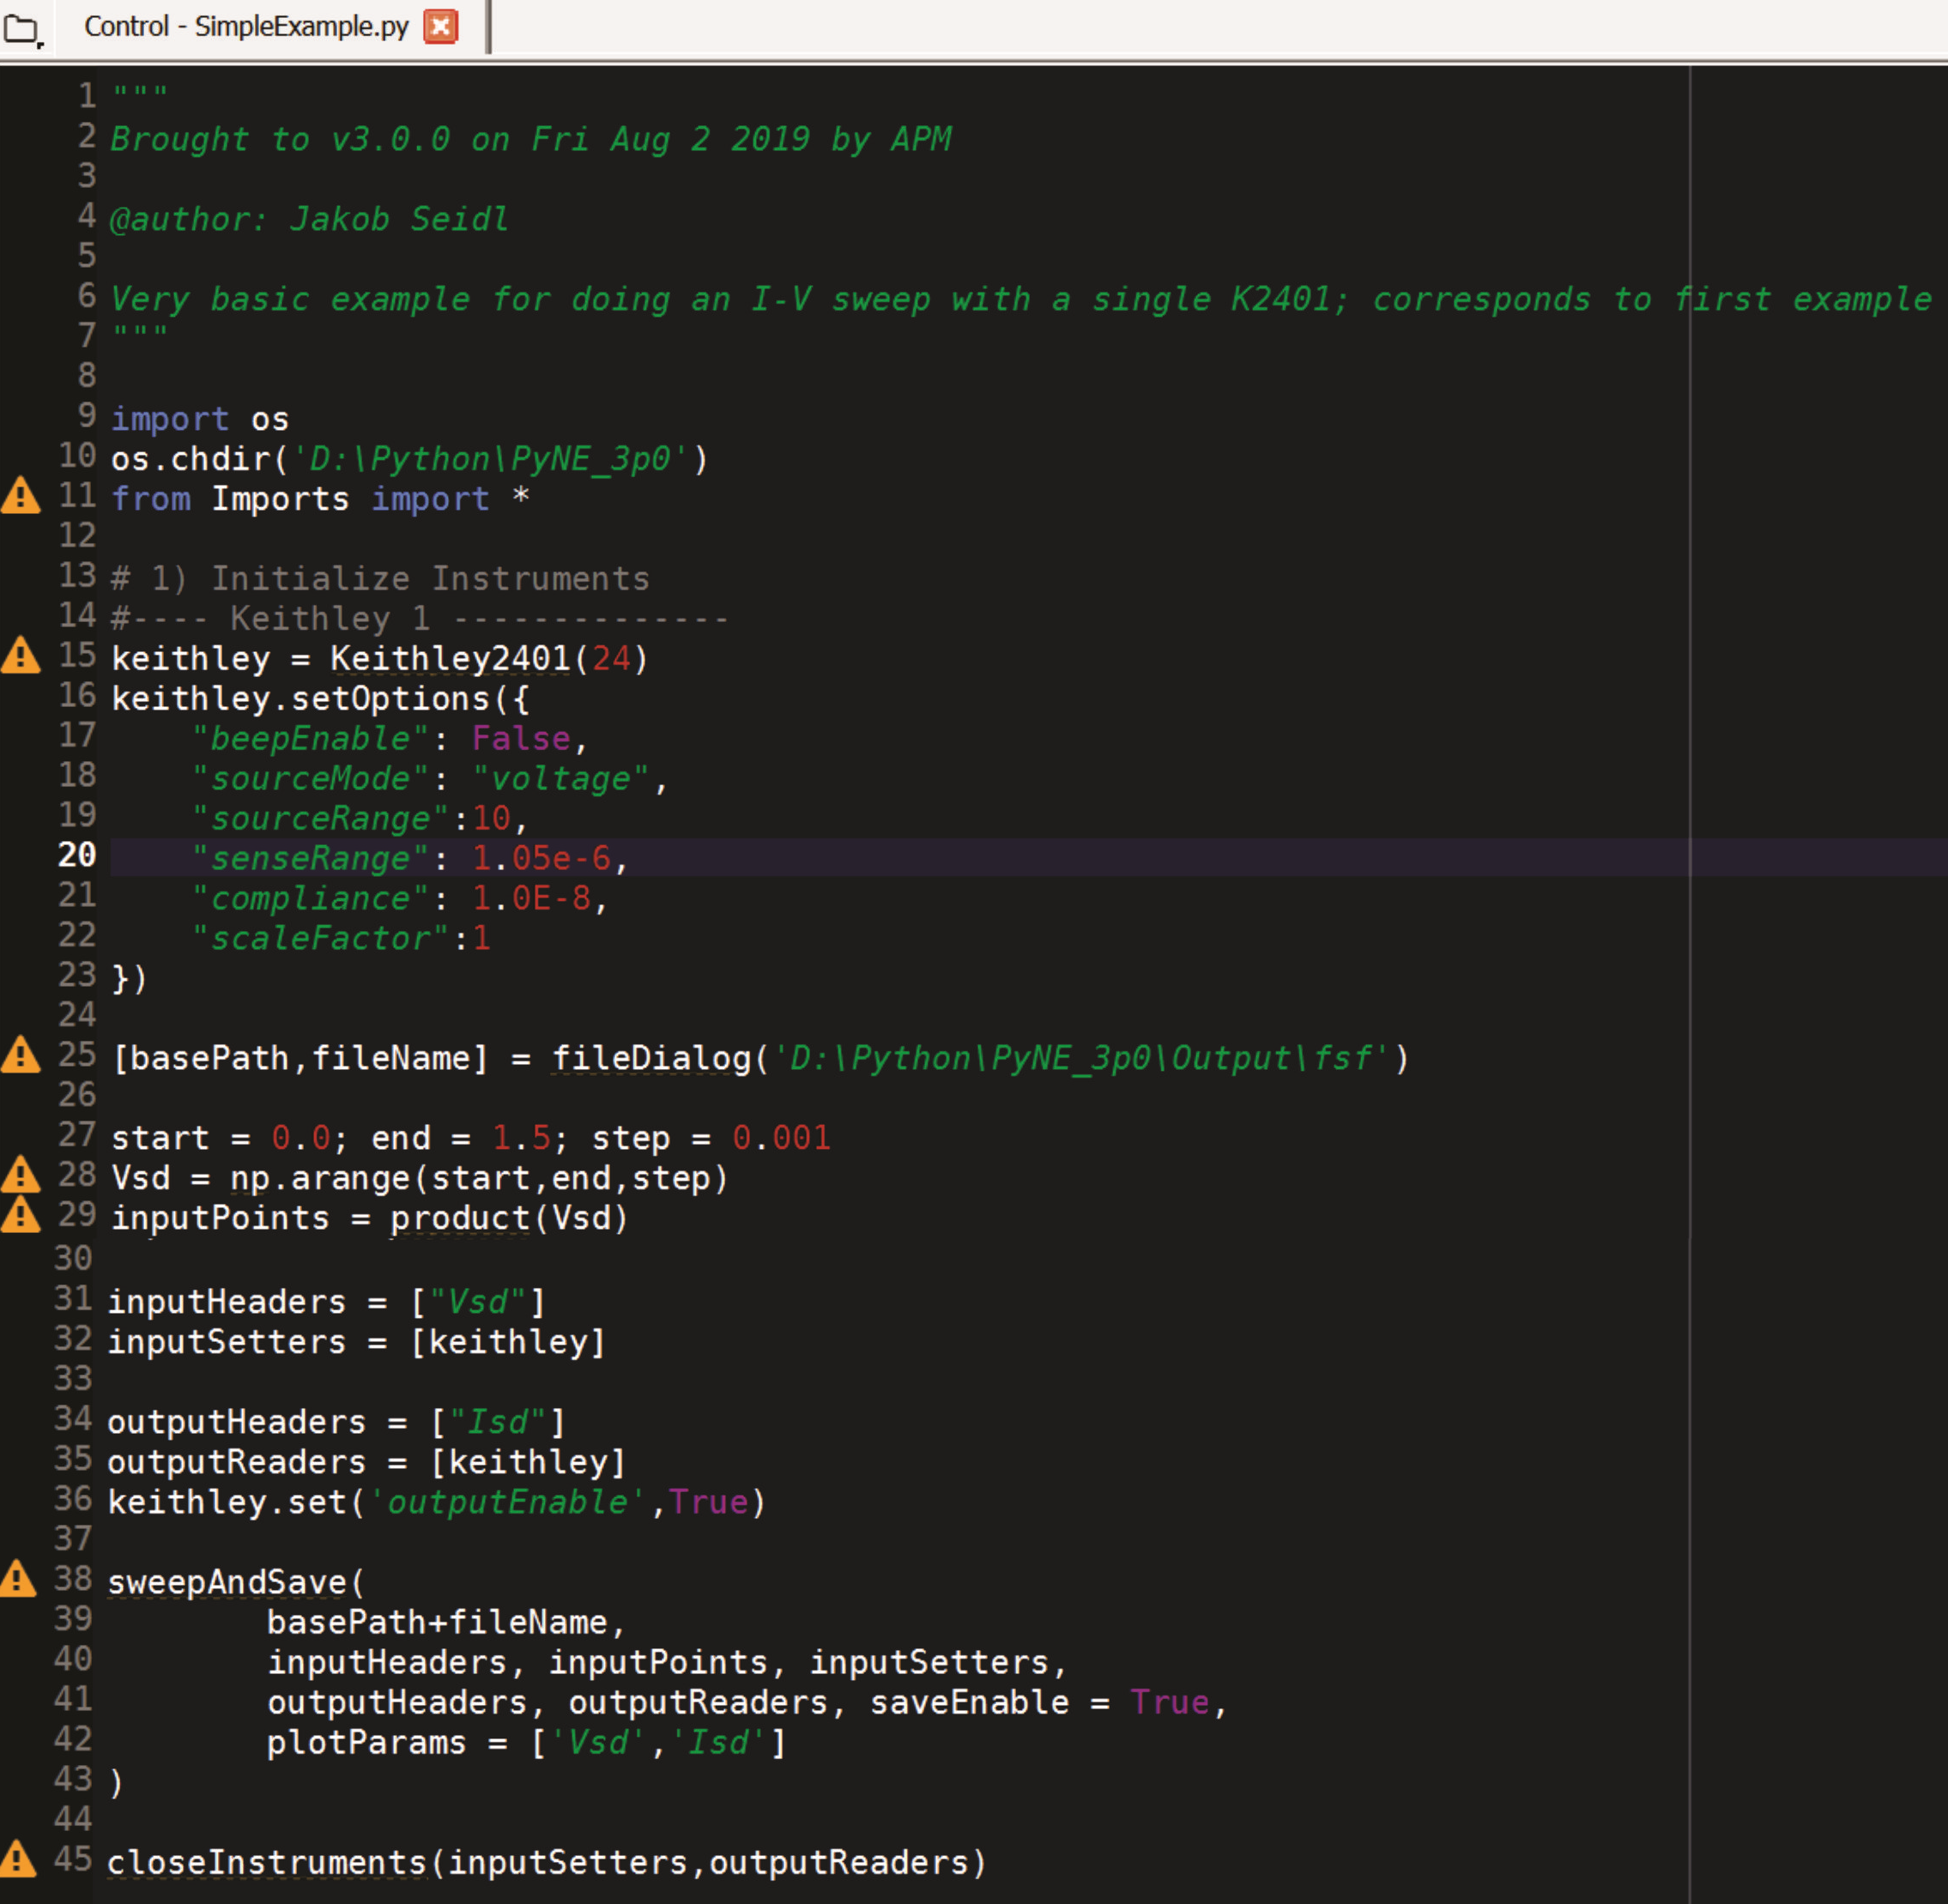
\includegraphics[width=16cm]{SimpleControl}
\caption{\textbf{Control workflow.} Lines 9-11 import the required functions. Lines 15-23 define an instrument and set the measurement options. Line 25 calls a GUI for selecting the results directory and file name. The array of data points we want to sweep over is defined in Lines 27-28 and converted into a suitable format in Line 29. Lines 31-36 show the setup of input and output headers $\textsf{\&}$ setters (see text). After the output of the SMU is enabled in Line 36, the main sweep function is called in Lines 38-43. Finally, all instrument connections are closed in Line 35.}
\label{Fig:SimpleControl}
\end{figure}

In the next section, the Keithley2401 instrument is defined and connected via the command:\\

\begin{verbatim}
keithley = Keithley2401(24)
\end{verbatim}

In pyNE, instruments themselves are `instances' of the corresponding instrument type, which are represented by `classes'. If you are reading this, you may well be new to Object Oriented Programming (OOP) as well as Python, so that last sentence will be unintelligible. This footnote\footnote{The links on OOP are: https://www.freecodecamp.org/news/object-oriented-programming-concepts-21bb035f7260/ and https://www.makeuseof.com/tag/object-oriented-programming-explained/} has some links on the basic concept of object oriented programming. This footnote\footnote{The link on basics of python is: https://swcarpentry.github.io/python-novice-inflammation/} has a good way to start learning the very basics of Python (albeit using Jupyter notebooks, but the syntax is very similar). So, assuming you now know at least the basic OOP concept, let's get back to it. Upon creation of an instrument instance, you only have to specify the instrument type (here Keithley2401) and GPIB address (here 24). You can create multiple instruments (instances) of the same type by repeating the above command using a different name and GPIB address, e.g., like this:\\

\begin{verbatim}
keithley1 = Keithley2401(24)
keithley2 = Keithley2401(11)
\end{verbatim}

There are only two instruments presently that violate this rule. The first is the `time' instrument, which takes as its argument the time interval rather than the GPIB. The second is the NI USB-6216, which takes as its argument the port number you want to control. The reason for this is that neither of these instruments is on the GPIB bus. More details on this in Section~2.\\

These instruments are instances of `classes' (see OOP footnote), which means you can use the rather convenient `dot notation', e.g., \texttt{keithley.goTo(0.0)}, to access the corresponding class functions, which are instrument operations, settings or parameters. Some of these functions are the most basic instrument functionalities you could access from their front panels, e.g., enable or disable output voltage. The software also provides some higher level functions that can execute sequences of low-level functions for you. In the example in Fig.~1.1, in Lines 16-23, we use the function below:\\

\begin{verbatim}
keithley.setOptions({
    "beepEnable": False,
    "sourceMode": "voltage",
    "sourceRange":10,
    "senseRange": 1.05e-6,
    "compliance": 1.0E-8,
    "scaleFactor":1
})
\end{verbatim}

to set a bunch of instrument options all at once. Every instrument has this function but the available options naturally vary from instrument to instrument. The options are formatted in python dictionary format, i.e., consist of a \texttt{`key'} with a corresponding \texttt{`value'}. A comprehensive list of all implemented options can be found in Section~2.\\
\\
Line 25 opens a short GUI (Graphical User Interface) dialog window, where a user specifies the desired base folder and filename for saving their data. These are saved in the variables `basePath' and `fileName', which can be overwritten manually via a later line in the code if needed, e.g., in order to give certain sweeps completely different filename structure.\\
\\
After all instruments are properly initialized, we can begin to define the parameter space we'd like to sweep through. The \textit{numpy arange}\footnote{\textit{numpy} is commonly imported as `np' in the python community and we stick to this convention.} is a convenient way of defining an equally spaced array ranging from a start to and end value\footnote{Note that np.arange by default excludes the endpoint - this is why Adam often prefers np.linspace, which has an endpoint = True/False option}, c.f. Lines 27-28. For a few discrete points, it might be better to use a simple python list like `Vsd = [0.2, 0.3, 0.5]' instead. The next line, Line 29, converts this newly defined array/list into the format required by the function that performs the actual sweep. It creates an \textit{itertools.product} `object' in the SweepFunction.py routine. For a single parameter sweep, like we do here, the product object will simply be a 1D array. However, when provided two or more inputs, this command will create a product array comprised of all the inputs. To give an example, say you'd like to perform a simple gatesweep measurement for a set of source-drain biases. You'd define the gatesweep range (Vg) using np.arange just like in the example code but additionally define `Vsd = [0.2, 0.3, 0.5]', for example. Then \texttt{InputPoints = product(Vsd,Vg)} would span your entire (2D) parameter space, i.e., do one full Vg sweep for Vsd$ = 0.2$~V, one for $0.3$~V and one for $0.5$~V. The order in which the inputs are placed matters, it governs the sweep order, so be careful about how this is assembled. The keyword \texttt{inputPoints} has been established as the keyword for the final array. This is just a name though and can be changed if needed.\\
\\
After initializing the instrument(s) and setting the sweep parameter space, we can now declare which of these instruments are going to actually do the sweep, i.e., set parameters (referred to as \textit{setters}) and which instruments will measure data (\textit{readers}). At the same time we also define how we want to call the parameters that are sourced or acquired. This is done via the \textit{headers} that exist for the swept variables (\textit{inputHeaders}) and measured data (\textit{outputHeaders}). If you have multiple instruments you define these via a simple list, e.g., inputSetters = [keithley,yokogawa]; the same holds for the corresponding headers. Make sure that the order in which the headers and setters are defined matches. The first setter will always be identified with the first header and so forth; avoid errors here since they will, at the least, create a lot of confusion in your data files. Some instruments return two values when measuring, e.g., lock-in amplifiers, you should use additional brackets [...] to denote this pair of variables, like this:\\

\begin{verbatim}
outputHeaders = [[Ix,Iy],GateLeakage]
outputReaders = [LockIn1,Keithley_Vg]
\end{verbatim}

Finally, after declaring input and output instruments and variables, we then pass all these variables to the main function \textit{sweepAndSave}, which performs the sweep:\\

\begin{verbatim}
sweepAndSave(
    basePath+fileName,
    inputHeaders, inputPoints, inputSetters,
    outputHeaders, outputReaders,saveEnable = True,breakCondition = breakCond,
    plotParams = ['Vsd','Isd']
)
\end{verbatim}

Let's quickly go through the input variables:\\

\begin{enumerate}
\item The full file path. Note that strings can just be added in python and thus basePath+fileName is just a string.
\item inputHeaders, inputPoints and inputSetters. These variables were defined above and specify instruments and values that are actively sourced.
\item outputHeaders, outputReaders. As defined above, these specify all instruments and quantities that are read/measured.
\item saveEnable is a boolean (True or False) that decides whether the obtained data will be saved (as .tsv, .mat and .png file) or not.
\item breakCondition = breakCondition is still in the making and not yet implemented. Please leave this out for now.
\item plotParams denotes the variables among inputHeaders and outputHeaders that you want to get plotted while measuring. Currently, you can only specify two pairs of variables, i.e., obtain two live plots. Note also that the first variable is always plotted on the \textit{x}-axis and must come from the \texttt{inputHeaders} while the second is on the \textit{y}-axis and should be chosen from the range of \texttt{outputHeaders}.
\end{enumerate}

The sweepAndSave() function will do the rest, i.e., slowly sweep all the setters to their initial sweep point (to avoid abrupt changes) and then carry out the sweep. Finally,\\

\begin{verbatim}
closeInstruments(inputSetters,outputReaders)
\end{verbatim}

will close the connection to all your instruments, as long as they are included in either inputSetter or outputReaders. You can also manually close any instrument by typing:\\

\begin{verbatim}
instrument.close()
\end{verbatim}

\section{A more complex example - combining measurements}
Having seen how to construct a simple measurement in our control file, it is time to move on to a more sophisticated example. Here we will combine \textit{$I_d$ vs. $V_{sd}$} measurement with a set of subsequent \textit{$I_d$ vs. $V_g$} gatesweeps.\\

\scriptsize
\begin{verbatim}
import os
os.chdir('D:\Python\PyNE_3p0')
from Imports import *

#----Keithley Vsd --------------
Ksd = Keithley2401(24)
Ksd.setOptions({
    "beepEnable": False,
    "sourceMode": "voltage",
    "sourceRange":1,
    "senseRange": 1.05e-5,
    "compliance": 1.0E-5,
    "scaleFactor":1
})

#---Keithley Vg -----------
KVg = Keithley2401(11)
KVg.setOptions({
    "beepEnable": False,
    "sourceMode": "voltage",
    "sourceRange":1,
    "senseRange": 1.05e-6,
    "compliance": 1.0E-7,
    "scaleFactor":1
})

#Electrometer
eMeter = Keithley6517A(20)
eMeter.setOptions({
    "autoRange":True,
    "senseRange":2E-6,
    "senseMode":"current",
})

[basePath,fileName] = fileDialog()

#Vsd array
start = -0.05; end = 0.5; step = 0.001 #Create a up and downsweep array
VsdUp = np.arange(start, end, step) #Only the upsweep
VsdDown = np.arange(end, start-step, -step)
VsdUpDown = np.concatenate((VsdUp, VsdDown)) #np.concatenate() fuses two arrays to one

#Gatesweep array, Vg
start = 0.0; end = 1.4; step = 0.005 #Create a up and downsweep array
Vg = np.concatenate(( #np.concatenate() fuses two arrays to one
        np.arange(start, end, step),
        np.arange(end, start-step, -step)
))

#--------------Headers and setters for IV curves
inputHeaders = ["Vsd"]
inputSetters = [Ksd]
outputHeaders = ["Id","Idrough"]
outputReaders = [eMeter,Ksd]
Ksd.set('outputEnable',True)
for i in range(3): # 3 Vsd sweeps from -0.05 -> 0.05 V
    inputPoints = product(VsdUpDown)
    sweepAndSave(
            basePath+fileName,
            inputHeaders, inputPoints, inputSetters,
            outputHeaders, outputReaders,saveEnable = True,
            plotParams = ['Vsd','Id']
    )
Ksd.goTo(0.05,delay=0.001) # since we stop the sweep at -0.05 V we go to 0.05 V manually

#--------------Headers and setters for Vg curves
inputHeaders = ["Vg"]
inputSetters = [KVg]
outputHeaders = ["Id","Ileak","Idrough"]
outputReaders = [eMeter,KVg,Ksd]
for i in range(5): # do 5 full gatesweeps from 0 to 1.4 V
    inputPoints = product(Vg)
    sweepAndSave(
            basePath+fileName,
            inputHeaders, inputPoints, inputSetters,
            outputHeaders, outputReaders,saveEnable = True,
            plotParams = ['Vg','Id','Vg','Ileak']
    )

Ksd.goTo(0.00,delay=0.001)

closeInstruments(inputSetters,outputReaders)
\end{verbatim}
\normalsize

Here, we import three instruments: two Keithley2401 source-measure units (SMUs) and one Keithley6517A electrometer. After setting their options, we define arrays for both the gate voltage $V_{\mathrm{g}}$ and the source-drain bias $V_{\mathrm{sd}}$. The \texttt{np.concatenate()} function is used to join two arrays into one. This allows for up and downsweeps using just one array or using a higher point-spacing in certain parts of the sweep than in others.\footnote{For example, you could have a coarse spacing in the uninteresting regions of a gatesweep and a fine resolution in an interesting region.} Note that the headers and setters must be defined separately for each measurement, since different instruments are sourcing the voltages/currents in each of these measurements. You might also want to measure a separate set of variables, and name them differently, and this is possible with this structure.\\
\\
Two last things we'd like to draw your attention to:\\
Any setter instrument can be swept to any (sensible) value using:\\

\begin{verbatim}
instrument.goTo(targetValue,stepsize,delay)
\end{verbatim}

This is the same command we use before performing the gate sweep in order to sweep the source-drain bias back from $-0.05$~V to $0.05$~V. Note also the use of \textit{for loops} in this script. These provide a very simple control over how many times we'd like to perform a sweep. One could in principle combine \textit{for} and \textit{while} loops with different conditions based on measurement outcomes to creating more sophisticated measurement routines, e.g., sequence of repeated measurements that self-terminates once one of the parameters crosses a threshold.\\




\chapter{Instruments, Functions and Ranges}

\lettrine[lines=2]{\color{blue}\textsf{I}}{}n this chapter, we will introduce all available instruments with their unique options and measurement ranges. It may hopefully provide a useful day to day companion when coding your control file. All the properties with their \texttt{"key"} are accessible via the \texttt{instrument.set("key",value)} or \texttt{instrument.setOptions($\lbrace$"key1":value1, "key2":value2 $\rbrace $} functions.

\section{Keithley 2401}

\textbf{\textsf{Short description}:} Keithley source-measure unit. Is able to source a voltage/current while reading the current/voltage that it puts out at the same time. Standard unit in the fishtank lab.\\
\textbf{\textsf{Setter or reader}:} Both\\
\textbf{\textsf{Sourcemode} (\texttt{"sourceMode"}):} Selects the current or voltage sourcemode. Also internally sets the senseMode: The K2401 will measure current when sourcing voltage and vice versa.\\
\textbf{\textsf{Source ranges} (\texttt{"sourceRange"}):}
\begin{itemize}[noitemsep]
\item \textbf{\textsf{Voltage:}} [20, 10, 1, 0.1, 0.01, 0.001] V\\
\item \textbf{\textsf{Current:}} [1, 0.1, 0.01, 0.001, \SI{1E-4}, \SI{1E-5}, \SI{1E-6}] A\\
\end{itemize}
\textbf{\textsf{Sense/Measurement ranges} (\texttt{"senseRange"}):}
\begin{itemize}[noitemsep]
\item \textbf{\textsf{Sensing voltage:}} [21.00, 2.10, 0.21] V\\
\item \textbf{\textsf{Sensing current:}} [\SI{1.05E-4}, \SI{1.05E-5}, \SI{1.05E-6}] A
\end{itemize}
The current sensing ranges go even higher (will be implemented soon), just remember that you might have to increase the compliance if you'd like to increase the sensing range - they are linked (see below in the compliance section).\\
\textbf{\textsf{Compliance} (\texttt{"compliance"}):}
\begin{itemize}[noitemsep]
\item \textbf{\textsf{Sensing current:}} [\SI{1.0E-9}, \SI{1.0E-8}, \SI{1.0E-7}] $\rightarrow$ 1.05$\;$A. \\
\item \textbf{\textsf{Sensing voltage:}} [\SI{0.2E-3}, \SI{2E-3}, 0.02] $\rightarrow$ 21$\;$V.\\
\end{itemize}
Note, the "senseRange" limits the lower compliance bounds and thus three values are given each, i.e. [lowerBound1, lowerBound2, etc.] $\rightarrow$ upperBound.\\
\\
\textbf{\textsf{Beep enable} (\texttt{"beepEnable"}):} Boolean. Enables (True) or disables (False) the annoying Keithley beep when an error occurs. Important when debugging.\\
\textbf{\textsf{Output enable} (\texttt{"outputEnable"}}): Boolean. Enables (True) or disables (False) source output. Reading the instrument with output off will result in an error since the instrument is basically off.\\
\textbf{\textsf{Scale factor} (\texttt{"scaleFactor"}}): You can introduce an additional scale factor if you use e.g. a current to voltage amplifier with a known amplification. The instrument will put out the measured value divided by the scale factor. By default, this factor is 1.

\section{Keithley 6517A Electrometer }

\textbf{\textsf{Short description}:} Keithley electrometer/High resistance meter. Able to precisely measure currents down to the few pA range. \\
\textbf{\textsf{Setter or reader}:} Reader only (for now).\\
\textbf{\textsf{Sensemode} (\texttt{"senseMode"}):} Selects the current or voltage sensing mode.\\
\textbf{\textsf{Sense/Measurement ranges} (\texttt{"senseRange"}):}
\begin{itemize}[noitemsep]
\item \textbf{\textsf{Sensing voltage:}} [2, 20, 200] V\\
\item \textbf{\textsf{Sensing current:}} [\SI{20E-12}, \SI{200E-12}, \SI{2E-9}, \SI{20E-9}, \SI{200E-9}, \SI{2E-6}, \SI{20E-6}, \SI{200E-6}, \SI{2E-3}, \SI{20E-3}] A
\end{itemize}
\textbf{\textsf{Zerocheck} (\texttt{"zeroCheck"}):} Boolean. Enables (True) or disables (False) zerocheck option on the electrometer. Zerocheck basically put a large resistor in line with the measurement line when enabled, thus decreasing the current flow and mitigating possible damage to the sensitive instrument.\\
\textbf{\textsf{Autorange} (\texttt{"autoRange"}):} Boolean. Enables (True) or disables (False) the autorange pyNE function.\\

\section{Yokogawa GS200}

\textbf{\textsf{Short description}:} Power supply known for its low noise. No real measure capabilities. \\
\textbf{\textsf{Setter or reader}:} Setter only.\\
\textbf{\textsf{Sourcemode} (\texttt{"sourceMode"}):} Selects the current or voltage sourcing mode.\\
\textbf{\textsf{Source ranges} (\texttt{"sourceRange"}):}
\begin{itemize}[noitemsep]
\item \textbf{\textsf{Sourcing voltage:}} [0.01, 0.1, 1, 10, 30] V\\
\item \textbf{\textsf{Sourcing current:}} [0.001, 0.01, 0.1, 0.2] A
\end{itemize}
\textbf{\textsf{Compliance} (\texttt{"compliance"}):}
\begin{itemize}[noitemsep]
\item \textbf{\textsf{Sourcing voltage:}} 0.001 $\rightarrow$ 0.1$\;$A\\
\item \textbf{\textsf{Sourcing current/sensing voltage:}} 1 $\rightarrow$ 30$\;$V
\end{itemize}
The YokogawaGS200 only accepts current protection for the 30, 10 and 1$\,$V voltage ranges.\\

\section{SR(S)830 Lock-In Amplifier}

\textbf{\textsf{Short description}:} Lock-in amplifier with a oscillator frequency of up to ca. 100kHz.\\
\textbf{\textsf{Setter or reader}:} Can act as both.\\
\textbf{\textsf{Time constant} (\texttt{"timeConst"}):} Sets the time constant over which the lock-in integrates.\\
\begin{itemize}[noitemsep]
\item \textbf{\textsf{Possible time constants:}} [\SI{10E-6}, \SI{30E-6}, \SI{100E-6},\SI{300E-6}, \SI{1E-3}, \SI{3E-3}, \SI{10E-3}, \SI{30E-3}, \SI{100E-3},\SI{300E-3},1, 3, 10, 30, 100, 300] seconds.
\end{itemize}
\textbf{\textsf{Sensitivity} (\texttt{"senseRange"}):} Sets the sensitivity of the measurement circuitry.\\
\begin{itemize}[noitemsep]
\item \textbf{\textsf{Sensitivities}:} [\SI{1E-9}, \SI{2E-9}, \SI{5E-9}, \SI{10E-9}, \SI{20E-9}, \SI{50E-9}, \SI{100E-9}, \SI{200E-9}, \SI{500E-9}, \SI{1E-6}, \SI{2E-6}, \SI{5E-6}, \SI{10E-6}, \SI{20E-6}, \SI{50E-6}, \SI{100E-6}, \SI{200E-6}, \SI{500E-6}, \SI{1E-3}, \SI{2E-3}, \SI{5E-3}, \SI{10E-3}, \SI{20E-3}, \SI{50E-3}, \SI{100E-3}, \SI{200E-3}, \SI{500E-3}, 1] V/$\mu$A.
\end{itemize}
Note that the user input always refers to the voltage input, i.e., the voltage scale used. The conversion between current and voltage scale is: current scale = voltage scale $\times 10^{-6}$\\
\\
\textbf{\textsf{Input} (\texttt{"input"}):} Sets the input used for the amplifier. In general, the lock-in can either measure voltage or current. There are two current inputs with different amplification factors ($10^6$, $10^8$) as well as a normal and a differential ('A-B') voltage measurement.\\
\begin{itemize}[noitemsep]
\item \textbf{\textsf{Available inputs:}} ['A', 'A-B', 'I1', 'I2'].
\end{itemize}
\textbf{\textsf{Frequency} (\texttt{"frequency"}):} Changes the frequency of the sine wave excitation output. Must be in [1, 100 000] Hz.\\
\textbf{\textsf{Amplitude} (\texttt{"amplitude"}):} Changes the amplitude of the sine wave excitation output. Must be in [0.004, 1] V.\\
\textbf{\textsf{Sweep parameter} (\texttt{"sweepParameter"}):} This option decides which lock-in parameter is swept in case it is used as a \texttt{setter} in a sweep function. This is necessary since there is no obvious choice. So far, it is possible to sweep the excitation frequency or the sine excitation amplitude.\\
\begin{itemize}[noitemsep]
\item \textbf{\textsf{Available parameters}: } ['frequency', 'amplitude'].
\end{itemize}
\textbf{\textsf{Sweep delay} (\texttt{"sweepDelay"}):} Sets the delay between each sweep iteration of aforementioned sweep parameter in seconds. Default is $0.5$~s.\\
\textbf{\textsf{Scale factor} (\texttt{"scaleFactor"}}): You can introduce an additional scale factor if you use, e.g., a current to voltage pre-amplifier with a known gain. The instrument will put out the measured value divided by the scale factor. By default, this factor is 1.\\
\textbf{\textsf{Auto sensitivity} (\texttt{"autoSensitivity"}):} Boolean. Enables (True) or disables (False) the autorange pyNE function.\\

\section{TimeMeas}

\textbf{\textsf{Short description}:} This is a virtual-instrument that either steps assigned wait periods or reports back the internal clock. Essentially there to enable time-sweeps.\\
\textbf{\textsf{Setter or reader}:} Can act as both.\\
You can assign the step interval in place of the GPIB address in the instrument call for setter function, or read back the time for reader function.\\

\section{USB-6216In}

\textbf{\textsf{Short description}:} DAC Input for the USB-6216, which is connected by USB. This is an unusual instrument in that it can currently be up to 10 instruments at once: 8 inputs and 2 outputs.\\
\textbf{\textsf{Setter or reader}:} Reader only. To set use USB-6216Out.\\
\textbf{\textsf{Address} (\texttt{0, 1, 2, 3, 4, 5, 6, 7}):} Sets which of the 8 available inputs will be assigned to the instrument.\\
\textbf{\textsf{inputLevel}:} Assigned call to return the inputVoltage on that line.\\
\textbf{\textsf{Scale factor} (\texttt{"scaleFactor"}}): You can introduce an additional scale factor if you use, e.g., a current to voltage pre-amplifier with a known gain. The instrument will put out the measured value divided by the scale factor. By default, this factor is 1.\\
\textbf{\textsf{Resolution}:} Not yet implemented, but will enable setting resolution for a given channel if fine scaling is required. Currently defaults to $+/-10$~V.\\

\section{USB-6216Out}

\textbf{\textsf{Short description}:} DAC Output for the USB-6216, which is connected by USB. This is an unusual instrument in that it can currently be up to 10 instruments at once: 8 inputs and 2 outputs.\\
\textbf{\textsf{Setter or reader}:} Setter and reader, but read returns current status of that line. To read only, use USB-6216In instead.\\
\textbf{\textsf{Address} (\texttt{0, 1}):} Sets which of the 2 available outputs will be assigned to the instrument.\\
\textbf{\textsf{outputLevel}:} Assigned call to set or return the outputVoltage on that line. What this is will depend on whether you set or read and your setting for feedback in the case of read.\\
\textbf{\textsf{feedBack} (\texttt{"Int" or "Ext"}):} Sets how the channel voltage state is read back\\
\begin{itemize}[noitemsep]
\item \texttt{"Int" :} Uses the internal connection inside the USB-6216 to directly read the voltage being put out on this line. This is the recommended option and the default.
\item \texttt{"Ext" :} Uses a specified analog input port to read the output voltage. This will require you to T- your output port and feed a BNC cable back to the relevant input. You will also need to specify which port this is. Defaults set to 6 and 7.
\end{itemize}
\textbf{\textsf{extPort}(\texttt{0, 1, 2, 3, 4, 5, 6, 7}):} Sets which of the 8 available inputs will be used to read the output voltage when you are in Ext mode. If using Int mode, this parameter is unused.\\
\textbf{\textsf{Scale factor} (\texttt{"scaleFactor"}}): You can introduce an additional scale factor if you use, e.g., a current to voltage pre-amplifier with a known gain. The instrument will put out the measured value divided by the scale factor. By default, this factor is 1.\\ 
\chapter{Installation and Setup}
What do you need in order to install the pyNE software package on a new computer? All the necessary installer files should be located in the 'Documentation/ Installers' directory.
\section{Prerequisites and installation}
\paragraph*{Anaconda}
We recommend using the \textbf{Anaconda 64-bit Python 3.7} distribution unless you are on an older machine running 32-bit OS. Anaconda contains almost all of the required scientific modules, e.g., \textit{numpy} and \textit{matplotlib} that pyNE requires internally to function. Smaller builds such as Miniconda, won't have these. There shouldn't be any 64-bit compatability issues unless you are using either very ancient NI GPIB hardware or an OS that doesn't support 64-bit. In either of these instances, you may want to return to pyNE for python 2.7 (original build).\\
\\
The Anaconda download will be an executable that will install the software in your system. You can find it at: https://www.anaconda.com/distribution/ but be sure to download the windows version (the page there tends to default to MacOS as the download). Follow the prompts, and run with its default options, it should be pretty straightforward. It is a good idea to install `for all users' if asked to ensure portability across users on the same machine. Once it is installed, you should reboot your system to ensure the environment \& dependencies are correctly set-up. Note: you can delay this reboot until after the next step if you need to install NI-VISA also.\\

\paragraph*{National instruments (NI) VISA libraries and drivers}
If these are not already on your machine, you will need to download and install these also. These can be found here: https://www.ni.com/en-au/support/downloads/drivers/download.ni-visa.html\#305862 We recommend installing as 64-bit unless your OS is still 32-bit or you are using extremely old NI hardware. Install using defaults, it is rather straightforward. After this step you should reboot your system to ensure the environment \& dependencies are correctly set-up.\\

\paragraph*{Install pyVisa and nidaq-mx libraries for python}
There are two python libraries that aren't in the standard Anaconda distribution that we need to add. The first is the python libraries for running NI Visa. The second are the libraries specific to the USB-6216 can National Instruments MAX (NI-MAX). The latter actually has two options, PyDAQmx and nidaqmx python API. I chose the latter as it's written/supported by NI, but if you want to use the former, you need to install that library using the same method below.
\begin{enumerate}
\item In the windows start screen search for 'Anaconda prompt'.
\item Right click on it and choose the 'Run as Administrator' option, then select yes when the OS acts you to confirm you want to run as admin. You need to use this option here, or the library install may fail due to access block issues.
\item A terminal should appear. To install pyVisa, type '\texttt{conda install -c conda-forge pyvisa}' and execute. This should automatically install the module with all its dependencies.
\item After this completes, follow up with '\texttt{conda install -c conda-forge nidaqmx}' to install the NIDAQ libraries. If you want PyDaqmx, you will need to install using pip as it's not presently supported by Conda-forge. You might want to talk to Adam about some of the issues here before proceeding.
\end{enumerate}

\paragraph*{Creating a base folder/path}. pyNE itself is only a collection of scripts and thus does not need to be installed as such. You just choose a suitable folder and copy the contents of the latest pyNE version into it. Write down the full path of this folder. Every \textit{control file} starts with importing these scripts via
\begin{verbatim}
import os
os.chdir('basefolder')
from Imports import *
\end{verbatim}
and you need to use the filepath where your pyNE scripts are located.

\paragraph*{Spyder IDE}
This is automatically installed with Anaconda. You run it from the same Anaconda prompt that you used to install the pyvisa and nidaqmx libraries (you don't need to be admin to run it, only for package installations). To do this, you type '\texttt{spyder}' and it should start up. An example screenshot is shown below.\\

\begin{figure}[h]
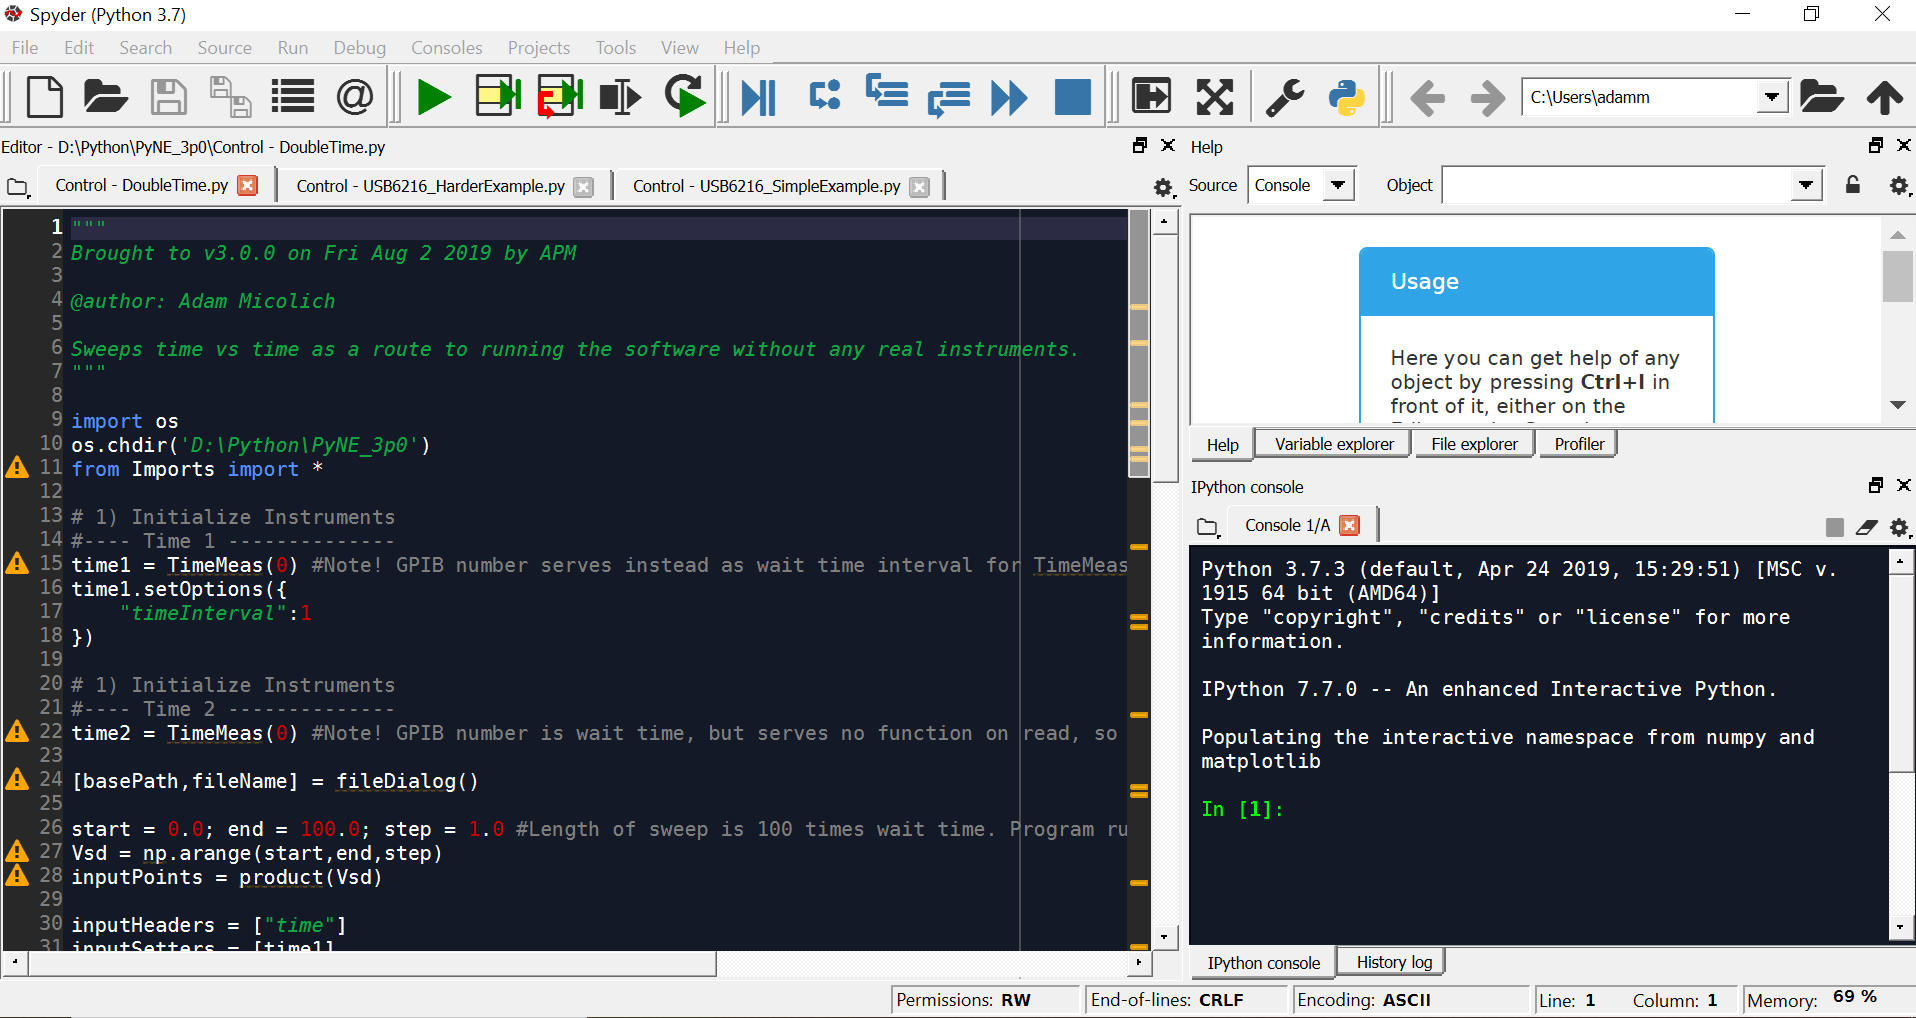
\includegraphics[width=16cm]{Spyder_screen}
\caption{\textbf{Spyder screenshot} Programs are loaded and edited on the left, the bottom right is your iPython console for running commands and seeing program output, the top right has panels for looking at contents of program variables, file structures, etc.}
\label{Fig:Spyderscreen}
\end{figure}

Figure~\ref{Fig:Spyderscreen} shows a screenshot of the Spyder IDE. You load your relevant control file, edit accordingly (even if it's just to set the operating directory), save and then execute using the green triangle in the top menu (run). A good test for this is to use the Control - DoubleTime.py file in the Examples directory, it is designed to be run on a computer without any instruments attached, since it uses the TimeMeas virtual instrument as both the control (setter) and output (reader) for the sweep. If it is working correctly, it should first bring up the GUI asking where to save the data file (see Section~1), and then put a graph to screen plotting time against time (trivial I know, but a good test for correct installation) and terminate.

\paragraph*{Setup the proper measurement ID file.}
Every measurement in pyNE has a running script consisting of a two letters and increasing number. For example, MeasurementNamePr123 would mean that the measurement 'MeasurementName' (which it takes from the GUI that comes up when you start a sweep) was the 123rd measurement on the Rack that is associated with the measurement setup Pr (in this case the probestation/gasbox).\\
\\
When initializing a new setup, we have to do two things: Set the counter back to zero and create a new letter combination associated with this new setup. To do this:\\
\begin{enumerate}
\item Open the GlobalMeasID.py file in spyder so you can edit its contents. Change the IDpath variable to 'basefolder\setminus GlobalMeasIDBinary'. Edit the \texttt{currentSetup} variable to a string of your choice. We recommend keeping it down to two letters for simplicity, e.g., 'Pr' for Probestation as in the example code.
\item Import GlobalMeasID in Spyder so you can access its functions in the console. If Spyder can't locate it, change the current working directory into your pyNE folder. Now execute GlobalMeasID.init(). This will set the internal counter to zero.
\end{enumerate}

An alternative way to set the counter to zero is just to open the GlobalMeasIDBinary file using Spyder and change the number to zero and then save. 
\chapter{Examples}
The pyNE 3.0 distribution has a folder called Examples that currently has five control files in it. These are example code to help new users test an installation or develop their own control programs. The five programs are:\\
\section{Control - DoubleTime.py}
This program executes a simple sweep of time versus time, in other words, it will set up two instruments, one of which is just 'delay assigned time' and the other which is 'return the time since initialising the time instrument'. In a graph, you will see a plot of the number of delay times (as written, steps of 1 from 0 to 100) and the time that delay step occurred, the graph should be linear (unless you do something that intermittently delays the program execution).\\
\\
This program is kind of pointless except that it enables you to test an installation without needing to have any instruments attached to your machine. It is also useful for a new user who wants to just 'work out how the hell you run this crazy pyNE thing' for the first time, without having to find a rack and set-up a dummy measurement.\\
\section{control - SimpleExample.py}
This program executes a basic $I$-$V$ sweep with a single Keithley 2401 source-measure unit. Best used with the SMU output connected to one BNC connector of a resistor box with the other BNC grounded (ground plug). This should give a linear $I$-$V$ as output.\\
\section{control - HarderExample.py}
This program is a proper multi-instrument set-up featuring two K2401s and a K6517A electrometer, which is the basic FET characterisation set-up used on the probe station. This is best used on a FET box (e.g., 2SK940 with $10$~kohm in series with the channel), with the K2401s connected to the source (GPIB 24) and gate (GPIB 11), and the electrometer connected to the drain (GPIB 20). The software will first generate a set of three $I_{SD}$ vs $V_{SD}$ curves at different $V_{G}$ and then generate a set of five $I_{SD}$ vs $V_{G}$ curves at different $V_{SD}$.\\
\section{control - USB6216SimpleExample.py}
This program executes a basic voltage sweep with the USB6216, and is essentially designed as a very quick test that the instrument is working properly with your computer and that the nidaqmx libraries are all functioning. You should make sure that the USB6216 is connected to the computer as Dev1 in NIMAX, if this is not the case (and you can't make it so), then you will need to edit both USB6216In.py and USB6216Out.py accordingly. If this is a frequent issue, let Adam know and he can add Device numbering as an option to the code.\\
\\
Before executing this program, use a BNC cable to connect analog output 0 (ao0) to analog input 0 (ai0). The software will run ao0 to $-1$~V, then sweep from $-1$~V to $+1$~V, then sweep from $+1$~V back to $-1$~V, and then silently ramp ao0 back to $0$~V before terminating. You will see two sweeps, and they should both be linear with slope 1 because you are just measuring the output back.\\
\section{control - USB6216HarderExample.py}
This program is designed to do a full FET characterisation using the USB6216, and is designed to be used on the 2SK940 FET box (i.e., 2SK940 with $10$~kohm in series with the channel). Before executing, you should make sure that ao0 is connected to the source, ao1 is connected to the gate and ai0 connected to the output of a Femto DLPCA-200 current preamp (gain $10^{5}$ and DC mode), which is fed by the drain.\\
\\
The program will execute a set of $V_{SD}$ traces from $0$~V to $+2$~V and back at six different $V_{G} = +2$, $+2.2$, $+2.4$, $+2.6$, $+2.8$ and $+3.0$~V. These graphs should show a linear $I_{SD}$ vs $V_{SD}$, which saturates at high $V_{SD}$. This saturation point moves to higher voltage with increasing $V_{G}$. The saturation current also increases with increasing $V_{G}$.\\

 

\printbibliography

\end{document} 